\chapter{Analysis}

\section{Format of relational algebra}

In this section we present relation algebra operators which are used as input of compiler:
\begin{enumerate}
\item Projection - we used extended projection $\phi_L$, which remove columns, compute new columns using expressions and rename columns

\item Table operator, which is leaf or algebra tree. For this operator we need to provide arguments like:
\begin{itemize}
\item table name
\item information about index, like name and columns
\item columns to read
\end{itemize}
\item Join - we used theta join $\Join_C$. Condition $C$ can be in following format:
\begin{itemize}
\item Empty and in this case join represent Cartesian product.
\item $a_1=b_1~and~a_2=b_2~and~a_3=b_3~and...and~a_n=b_n$, where $a_k$ belong to first relation and $b_k$ belongs to other relation.
\item $a_1\oplus b \ominus a_2$, where $a_1$ and $a_2$ belong one input and $b$ belongs to second input. $\oplus$ and $\ominus$ can be $<$ or $\leq$.

\end{itemize}

In addition to condition we need to specify output attributes of join. They can be from both input and we can optionally assign them new name, in case we need to work with two attributes but they have same name.

Other types or joins are not directly supported, but can be replace with cross join with following selection.
\item Anti join wasn't presented with other join algorithms. We denote it $\ltimes_C$ where $C$ is anti join condition. Output of expression $R \ltimes_C S$ is relation with tuples from $R$, for which doesn't exist any tuple is $S$ that satisfy condition. We can us join and anti join to express outer join:
\begin{itemize}
\item 
 $R\Join^\circ_C S= (R\Join_C S)\cup (R\ltimes_C S)$
\end{itemize}
To be precise we need to add columns contain $null$ to result of anti join.
 
Other use is to compute difference $R-S$. This can be rewritten as $R \ltimes_C S$, where $C$ equates attributes from $R$ with same called attributes in $S$. 
 
Advantages of using this attribute is, that we don't need outer join and difference, which will make working with algebra a little easier.

In implemented tool condition $C$ of anti join can be in following format:
\begin{itemize}
\item $a_1=b_1~and~a_2=b_2~and~a_3=b_3~and...and~a_n=b_n$, where $a_k$ belong to first relation and $b_k$ belongs to other relation.
\end{itemize}
In addition to that, we also need to specify output attributes of anti join and optionally assign them a new name. They can be only from first input relation.
\item Group operator $\gamma_L$, where L is non empty list of group attributes and aggregate functions. Supported aggregate functions are $min$, $max$, $sum$ and $count$. Function $avg$ is not supported but it can easily computed. All mentioned functions except $count$ take one attribute as input, function count has empty input. 

As we mentioned before, group operator is more general version of duplicate elimination. That's why we don't include duplicate elimination in our algebra.
\item Sort operator $\tau_L$, where $L$ is a non empty list of attributes with sort directions.
\item Union - $\cup$ is set union. In case we want to bag union we can compute set union and eliminate duplicate using grouping operator. Requirement is that both relations have same number of columns and they have same name.
\item Selection - we used selection as described in classic relational algebra.

\end{enumerate}

\section{Physical algorithms}

In this section we enumerate and describe algorithms which are generated to output. We assume that queries have enough memory and physical operators doesn't have to store intermediate result on hard drive.

Here is a list on algorithms:
\begin{itemize}
\item $Filter$ - this algorithm reads input tuples and outputs tuple satisfying given condition. Output doesn't have to be sorted same way as input.
\item $Filter$ keeping order - this algorithm reads input tuples and outputs tuple satisfying given condition. Output has to be sorted same way as input.
\item $Hash~group$ - operator group tuples and computes aggregate functions. Grouping is performed using hash table.
\item $Sorted~group$ - operator groups tuples and computes aggregate functions. Input has to be sorted by group attributes.
\item $Column~operations$ - this is an implementation of extended projection algebra node. 
\item $Cross~join$ - this operator computes product of two relations.
\item $Hash~join$ - computes join with equal conditions using hash table. 
\item $Merge~equijoin$ - this algorithm computes join with equal conditions. Input relations has to be sorted by join attributes. Algorithm creates join result merging sorted relations.
\item $Merge~non~equijoin$ - operator computes theta join with condition $a_1\oplus b \ominus a_2$, where $a_1$ and $a_2$ belong one input and $b$ belongs to second input. Signs $\oplus$ and $\ominus$ can be $<$ or $\leq$. Input relations has to be sorted by join attributes. Algorithm computes join merging relations.
\item $Hash~anti~join$ -  algorithm computes anti join with equal conditions of two relations using hash table.
\item $Merge~anti~join$ - algorithm computes anti join with equal conditions. Input relations has to be sorted by join attributes.
\item $Table~scan$ - operator scans whole table from hard drive.
\item $Scan~and~sort~by~index$ - operator scans whole table from hard drive using index. Output will be sorted by columns on given index.
\item $Index~Scan$ - this algorithm uses index to read only tuples satisfying given condition.
\item $Sort$ - this algorithm sorts input. Input can be presorted, in this case operator uses this information and sorts only by not yet sorted attributes.
\item $Union$ - this operator is bag union, it only append tuples from one relation to another.

\end{itemize}

\section{Architecture}
The architecture of implemented tool is displayed in figure~\ref{fig:compilerarchitecture}.

\begin{figure}[h!]
  \centering
    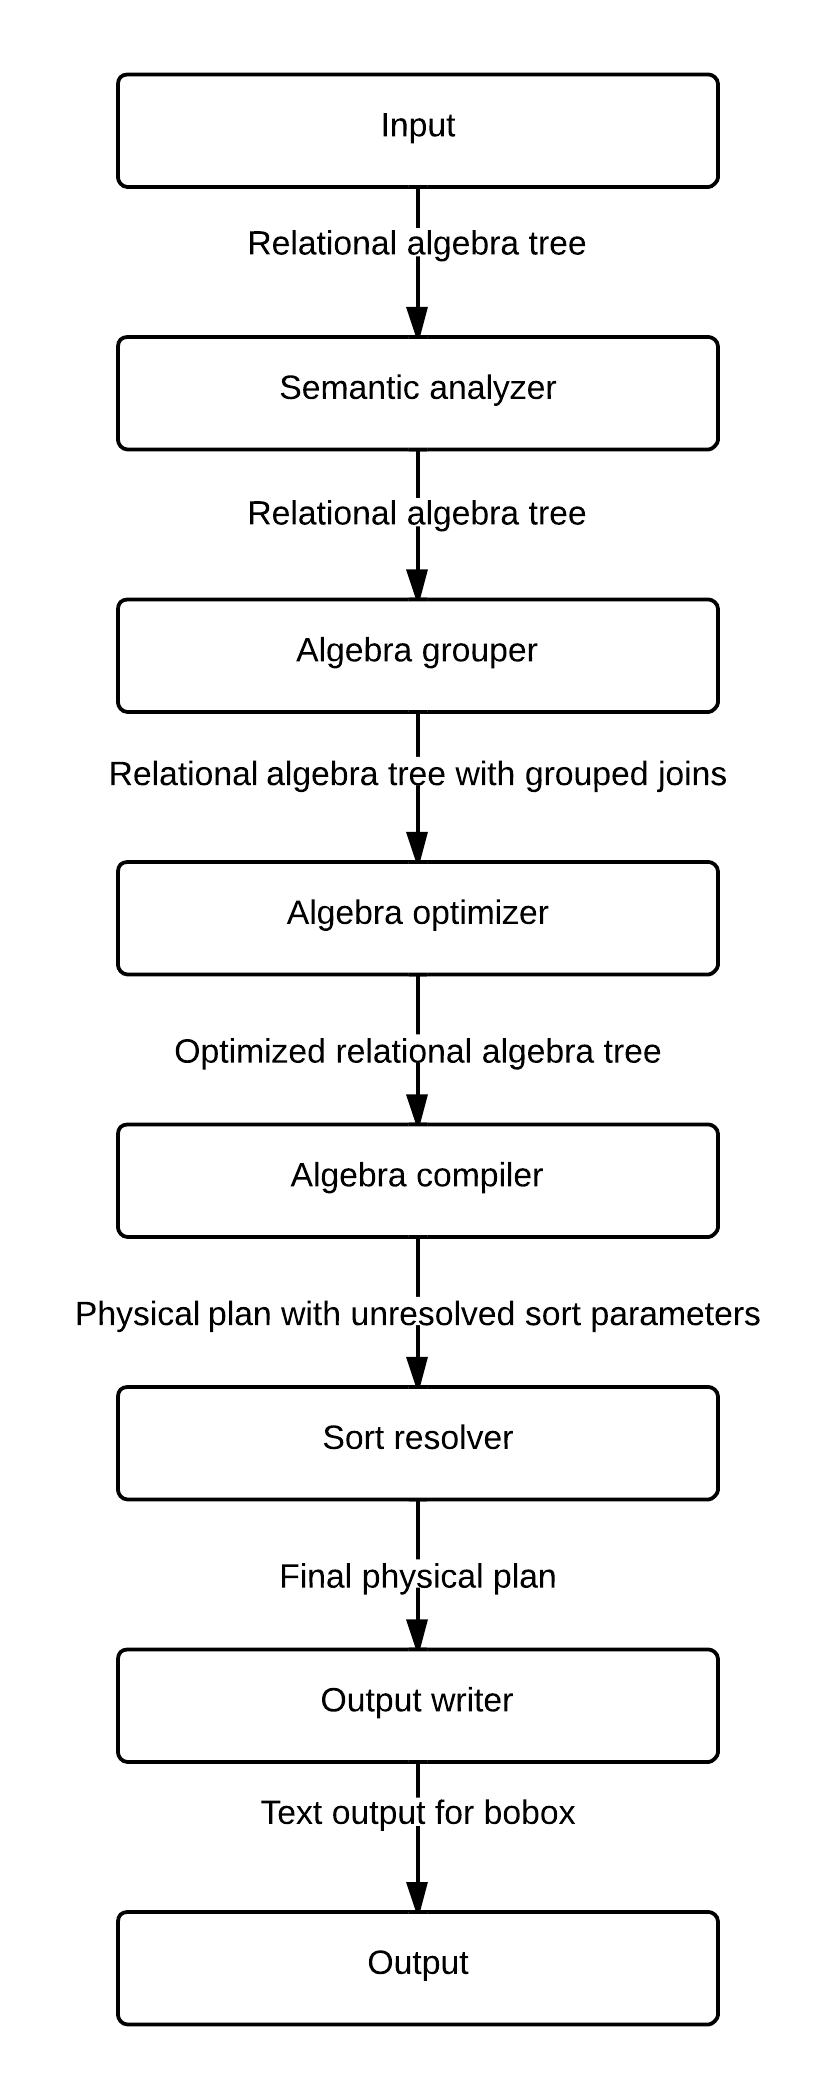
\includegraphics[width=0.5\textwidth]{compilerarchitecture}

      \caption{Compiler architecture.}
          \label{fig:compilerarchitecture}
\end{figure}

Relational algebra is read from input. the input is in XML format. For this format we decided for following reasons:
\begin{itemize}
\item XML has tree like structure exactly like relational algebra.
\item For validation we only need to write schema.
\item There are already implemented tools for parsing.
\item There is no need to write input parser.
\end{itemize}

After that relational algebra tree is checked in component called semantic checker. Semantic checker checks if all of used attributes are on input of operator or if there are no duplicate operators. 

Semantically correct tree goes to component that groups neighboring joins into one. This is done so we can choose fastest way to join multiple relations.

Algebra tree with grouped joins is optimized. We implemented one most important optimizations pushing selections down the tree. This component also pushes selection to join if selection contains equal condition, where one argument is from first and second argument is from second input.

Optimized algebra tree is processed by compiler, which generates physical plan which. This plan is not final. It's sort operator's parameters doesn't have to be final. For example if we want to sort relation before grouping we can sort it in different directions and than later decide what direction is better.

Final plan is output of component named Sort resolver. This component decides unknown sort order of sort operators.

Final plan is then converted to Bobolang in Output writer.

Implemented tool doesn't check types. Since it will be back end of compiler, the assumption is that front end parsing text will handle types. Types are only copied to output.

\section{Data structures}

\section{Optimization}

\section{Generating physical plan}




